\documentclass{article}%
\usepackage[T1]{fontenc}%
\usepackage[utf8]{inputenc}%
\usepackage{lmodern}%
\usepackage{textcomp}%
\usepackage{lastpage}%
\usepackage[head=40pt,margin=0.5in,bottom=0.6in]{geometry}%
\usepackage{graphicx}%
%
\title{\textbf{Avanzan en el desalojo y clausura de la planta de transferencia de Las Mayas}}%
\author{Diario El Universal}%
\date{21/09/2018}%
%
\begin{document}%
\normalsize%
\maketitle%
\textbf{URL: }%
http://www.eluniversal.com/caracas/21266/avanzan{-}en{-}el{-}desalojo{-}y{-}clausura{-}de{-}la{-}planta{-}de{-}transferencia{-}de{-}las{-}mayas\newline%
%
\textbf{Periodico: }%
EU, %
ID: %
21266, %
Seccion: %
caracas\newline%
%
\textbf{Palabras Claves: }%
NO\_TIENE\newline%
%
\textbf{Derecho: }%
3.2, %
Otros Derechos: %
, %
Sub Derechos: %
3.2.1\newline%
%
\textbf{EP: }%
NO\newline%
\newline%
%
\textbf{\textit{El plan está siendo ejecutado por el Minec en conjunto con el Gobierno del Distrito Capital y la Alcaldía del Municipio Libertador}}%
\newline%
\newline%
%
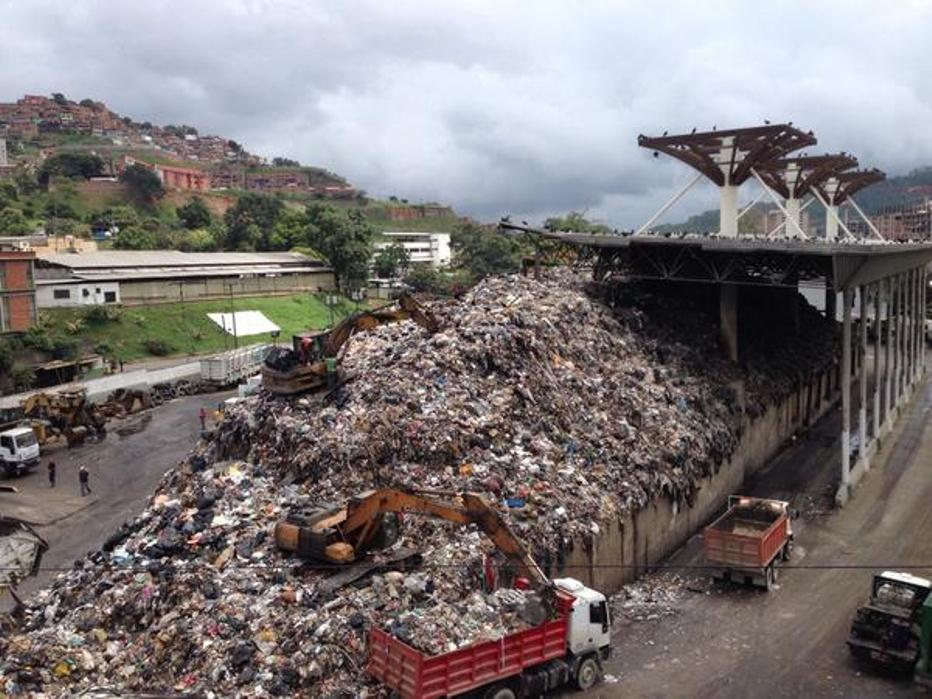
\includegraphics[width=300px]{129.jpg}%
\newline%
%
De acuerdo con las declaraciones ofrecidas por Heryck Rangel, Ministro del Poder Popular para el Ecosocialismo, se avanza en el proyecto de desalojo y clausura de la planta de transferencia de desechos sólidos Las Mayas.%
\newline%
%
Rangel manifestó que se verán beneficiados los habitantes de Coche, El Valle, Fuerte Tiuna y zonas aledañas.%
\newline%
%
El plan está siendo ejecutado por el Minec en conjunto con el Gobierno del Distrito Capital y la Alcaldía del Municipio Libertador.%
\newline%
%
El Ministro no ofreció detalles acerca del porcentaje de avance logrado hasta el momento ni la fecha de culminación de los trabajos%
\newline%
%
\end{document}